\section{Auswertung}
\label{sec:Auswertung}
\subsection{Einzelspalt}
Die aufgenommenen Messwerte zum Einzelspalt sind in der Tabelle \ref{tab:einzel} zu finden.
Zunächst wird die Position des Intensitätsmessgeräts $x$ in den Winkel $\phi$ umgerechnet.
Dafür wird $x$ zunächst um $x_0=  25.75\si{\milli\meter}$ verschoben.
Darauf wird eine Kleinwinkelnäherung
\begin{equation*}
    \phi \approx \tan{\phi} = \frac{x-x_0}{L}
\end{equation*}
durchgeführt, $L=0.85\si{\meter}$ entspricht hierbei dem Abstand von Spalt und Schirm.
Außerdem wird die der Dunkelstrom $I_\text{dun}$ von dem gemessenen Strom $I$ subtrahiert, da der Dunkelstrom nicht in die Auswertung mit einfließen soll.
Nun wird eine Ausgleichsrechnung mit der Gleichung \ref{eqn:beugungsfigur_parallel} durchgeführt.
Die Parameter $A_0$ und $b$ wurden dabei mit den Python Paket scipy \cite{scipy} berechnet.
Sie entsprechen den Werten
\begin{align*}
    A_0 &= \SI{8.154e-6}{}\\ 
    p_1 &= \frac{\lambda}{\pi b} = \SI{1.683}{\milli\meter}.
\end{align*}
Durch den Fitparameter kann nun die Spaltbreite $b$ bestimmt werden, sie beträgt $b = 0.1197 \si{\milli\meter}$.
Die Funktionen der Ausgleichsrechung wird zusammen mit den Messwerten sowie dem theoretischem Verlauf in Abbildung \ref{fig:einzel} dargestellt.
Zur Erstellung der Plots wurden die Python Pakete numpy \cite{numpy} und matplotlib \cite{matplotlib} genutzt.

\begin{figure}
    \centering
    
\includegraphics[width=\textwidth]{content/data/einzelspalt.pdf}
    \caption{Die Messwerte in Abhängigkeit von \phi, sowie der theoretische Verlauf und die durch Ausgleichsrechnung bestimmte Funktion.}
    \label{fig:einzel}
\end{figure}


%Messwerte Einzelspalt
\begin{table}
    \centering
    \begin{tabular}[t]{ccc|}
    \toprule
    $x\;/\; \si{\milli\meter}$ & $I_\text{dun}\;/\;\si{\nano\A}$ & $I \;/\; \si{\A}$\\
    \midrule
    0.0 & 0.40 & 5.5        \\
    2.0 & 0.50 & 5.6        \\
    4.0 & 0.52 & 7.8        \\
    6.0 & 0.52 & 7.5        \\
    8.0 & 0.50 & 6.1        \\
    10.0 & 0.56 & 12.0      \\
    11.0 & 0.50 & 15.5      \\
    12.0 & 0.52 & 11.5      \\
    13.0 & 0.50 & 14.1      \\
    14.0 & 0.52 & 32.1      \\
    15.0 & 0.54 & 54.0      \\
    16.0 & 0.46 & 41.1      \\
    17.0 & 0.52 & 26.0      \\
    18.0 & 0.50 & 73.5      \\
    19.0 & 0.50 & 160.0     \\
    20.0 & 0.50 & 120.0     \\
    20.5 & 0.42 & 72.0      \\
    21.0 & 0.40 & 32.5      \\
    21.5 & 0.44 & 82.0      \\
    22.0 & 0.48 & 420.0     \\
    22.5 & 0.44 & 900.0     \\
    23.0 & 0.44 & 2000.0    \\
    23.5 & 0.48 & 3400.0    \\
    24.0 & 0.54 & 5200.0    \\
    24.5 & 0.54 & 6600.0    \\
    25.0 & 0.60 & 7600.0    \\
    \bottomrule
    \end{tabular}
    \begin{tabular}[t]{|ccc}
    \toprule
    $x\;/\; \si{\milli\meter}$ & $I_\text{dun}\;/\;\si{\nano\A}$ & $I \;/\; \si{\A}$\\
    \midrule
    25.5 & 0.66 & 8000.0    \\
    26.0 & 0.58 & 8000.0    \\
    26.5 & 0.56 & 7300.0    \\
    27.0 & 0.55 & 6000.0    \\
    27.5 & 0.52 & 4800.0    \\
    28.0 & 0.56 & 3000.0    \\
    28.5 & 0.55 & 1820.0    \\
    29.0 & 0.57 & 820.0     \\
    29.5 & 0.56 & 340.0     \\
    30.0 & 0.58 & 120.0     \\
    31.0 & 0.56 & 240.0     \\
    32.0 & 0.54 & 325.0     \\
    33.0 & 0.54 & 180.0     \\
    34.0 & 0.50 & 39.0      \\
    35.0 & 0.52 & 56.5      \\
    36.0 & 0.49 & 100.0     \\
    37.0 & 0.50 & 78.0      \\
    38.0 & 0.50 & 20.0      \\
    39.0 & 0.50 & 17.0      \\
    40.0 & 0.54 & 39.0      \\
    42.0 & 0.48 & 30.0      \\
    44.0 & 0.48 & 26.0      \\
    46.0 & 0.46 & 14.0      \\
    48.0 & 0.44 & 10.0      \\
    50.0 & 0.46 & 14.5      \\
    \bottomrule
    \end{tabular}
    \caption{Der gemessene Dunkelstrom $I_\text{dun}$ und Strom $I$ bezüglich der Position $x$ des Intensitätsmessgeräts beim Einzelspalt.}
    \label{tab:einzel}
\end{table}
\FloatBarrier
\subsection{Doppelspalt}
Die Werte die bei der Messung des Interfernzmusters des Doppelspalts aufgenommen wurden sind in der Tabelle \ref{tab:doppel} zu finden.
Auch hier wird der Dunkelstrom $I_\text{dun}$ vom Strom $I$ subtrahiert.
$\phi$ wird wieder durch eine Kleinwinkelnäherung bestimmt.
Bei der Berechung des Winkels wurde $x_0 = 26 \si{\milli\meter}$ gewählt, sodass das Maximum bei $\phi = 0$ liegt.
Der Abstand zwischen Blende und Schirm wurde gemessen und beträgt $L = 85 \si{\centi\meter}$.
Nun wird wie zuvor zum Einzelspalt, auch für den Doppelspalt eine Ausgleichsrechung durchgeführt.
Diese wird mithilfe der Gleichung \ref{eqn:beugungsfigur_doppel} angefertigt.
Die Fitparameter
\begin{align*}
p_1 &= \frac{\lambda}{\pi b} = 0.00241\\
p_2 &= \pi \frac{s}{\lambda} = 160.23067 \\
\end{align*}
wurden wieder mit dem Python Paket scipy berechnet
Zusätzlich wird eine theoretischer Verlauf berechnet.
Der theoretische Verlauf, die Fit-Funktion und die Messwerte wurden anschließend in Abbildung \ref{fig:doppel} zusammengetragen.
\begin{figure}
    \centering
    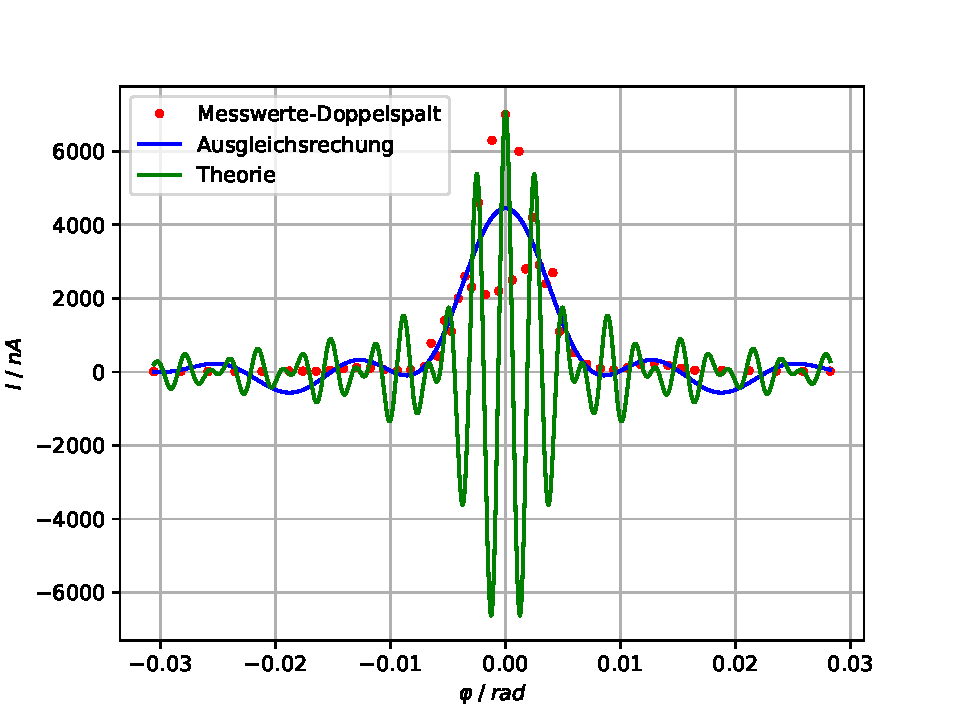
\includegraphics[width=\textwidth]{content/data/doppelspalt.pdf}
    \caption{Die Messwerte in Abhängigkeit von \phi, sowie der theoretische Verlauf und die durch Ausgleichsrechnung bestimmte Funktion.}
    \label{fig:doppel}
\end{figure}
Aus den Fitparametern ergibt sich für die Breite des Spaltes $b$ und die Abstand der beiden Spalten zueinander $g$ als
\begin{align*}
    b &= 0.82515\si{\milli\meter}\\
    g &= -0.79287 \si{\milli\meter} \\
\end{align*}
Der Abstand $g$ lässt sich durch $g = \frac{p_2\lambda}{\pi} -b$ berechnen.

\begin{table}
    \centering
    \begin{tabular}[t]{ccc|}
    \toprule
    $x\;/\; \si{\milli\meter}$ & $I_\text{dun}\;/\;\si{\nano\A}$ & $I \;/\; \si{\A}$\\
    \midrule
    0.0 & 0.38 & 10.0       \\
    2.0 & 0.42 & 14.0       \\
    4.0 & 0.46 & 9.8        \\
    6.0 & 0.40 & 7.8        \\
    8.0 & 0.42 & 16.0       \\
    10.0 & 0.44 & 24.0      \\
    11.0 & 0.42 & 20.0      \\
    12.0 & 0.38 & 18.0      \\
    13.0 & 0.40 & 42.0      \\
    14.0 & 0.42 & 92.0      \\
    15.0 & 0.44 & 120.0     \\
    16.0 & 0.42 & 100.0     \\
    17.0 & 0.42 & 58.0      \\
    18.0 & 0.42 & 34.0      \\
    19.0 & 0.42 & 56.0      \\
    20.0 & 0.40 & 140.0     \\
    20.5 & 0.44 & 780.0     \\
    21.0 & 0.44 & 430.0     \\
    21.5 & 0.42 & 1400.0    \\
    22.0 & 0.44 & 1100.0    \\
    22.5 & 0.46 & 2000.0    \\
    23.0 & 0.42 & 2600.0    \\
    23.5 & 0.42 & 2300.0    \\
    24.0 & 0.40 & 4600.0    \\
    24.5 & 0.44 & 2100.0    \\
    25.0 & 0.44 & 6300.0    \\
    \bottomrule
    \end{tabular}
    \begin{tabular}[t]{ccc|}
    \toprule
    $x\;/\; \si{\milli\meter}$ & $I_\text{dun}\;/\;\si{\nano\A}$ & $I \;/\; \si{\A}$\\
    \midrule

    25.5 & 0.41 & 2200.0    \\
    26.0 & 0.40 & 7000.0    \\
    26.5 & 0.40 & 2500.0    \\
    27.0 & 0.44 & 6000.0    \\
    27.5 & 0.44 & 2800.0    \\
    28.0 & 0.40 & 4200.0    \\
    28.5 & 0.44 & 2900.0    \\
    29.0 & 0.42 & 2400.0    \\
    29.5 & 0.44 & 2700.0    \\
    30.0 & 0.46 & 1100.0    \\
    31.0 & 0.44 & 520.0     \\
    32.0 & 0.40 & 210.0     \\
    33.0 & 0.46 & 90.0      \\
    34.0 & 0.38 & 50.0      \\
    35.0 & 0.44 & 110.0     \\
    36.0 & 0.38 & 200.0     \\
    37.0 & 0.41 & 240.0     \\
    38.0 & 0.40 & 180.0     \\
    39.0 & 0.40 & 100.0     \\
    40.0 & 0.40 & 46.0      \\
    42.0 & 0.38 & 41.0      \\
    44.0 & 0.34 & 34.0      \\
    46.0 & 0.39 & 19.0      \\
    48.0 & 0.44 & 13.0      \\
    50.0 & 0.42 & 20.0      \\
    \bottomrule
    \end{tabular}
    \caption{Der gemessene Dunkelstrom $I_\text{dun}$ und Strom $I$ bezüglich der Position $x$ des Intensitätsmessgeräts beim Doppelspalt.}
    \label{tab:doppel}
\end{table}